\documentclass[a4paper]{paper} 
\usepackage{babel}  
\usepackage[margin=2.5cm]{geometry}
\usepackage{graphicx}
\usepackage{xcolor}
\usepackage{booktabs}
\usepackage{microtype}
\usepackage{amsmath}
\usepackage{amsfonts}
\usepackage{natbib}
\renewcommand{\eqref}[1]{Eq.~(\ref{#1})}
\newcommand{\figref}[1]{Fig.~\ref{#1}}
\usepackage{libertine}
\usepackage{libertinust1math}
\usepackage[T1]{fontenc}
\usepackage{enumitem}
\sloppy

%% <---------------- fill according to your paper ----------------
\newcommand{\StudentName}{Zeeshan Ahmad}
\newcommand{\StudentMatrikelNumber}{23072973}
\newcommand{\PaperTitle}{MonoSDF: Exploring Monocular Geometric Cues for Neural Implicit Surface Reconstruction}
\newcommand{\AuthorList}{Zehao Yu, Songyou Peng and Andreas Geiger}
%% <--------------------------------------------------------------

\sectionfont{\large\sf\bfseries\color{black!70!blue}} 
\title{Seminar ``Inverse Rendering''}
\subtitle{Written Report\\
\hfill
\includegraphics[height=2.4cm]{fau-logo-right}
\vspace{-2cm}}
\author{\StudentName\\
\normalsize{Matrikel Number: {\StudentMatrikelNumber}}}
\begin{document} 
\twocolumn[\maketitle 
\textbf{\PaperTitle} \\ 
\AuthorList \\
\hrule\bigskip
]

%% <--------------------------------------------------------------
%% <--------------------------------------------------------------

\section{Introduction}
Digital Cameras project the 3D world onto a 2D image plane during rendering and lose 3D information including shape and texture. However, many real-world use cases require 3D information like robotics, animation, virtual reality, gaming, etc. Though various techniques have been proposed to solve this ill-posed inverse rendering problem but still it requires a lot more work. Current implicit surface reconstruction approaches work well for simple scenes and densely sampled scenes, however, they fail for large-scale scenes and few-shot reconstruction.\newline

This paper studies the effect of off-the-shelf monocular cues for 3D reconstruction combined with neural implicit scene representations to overcome reconstruction ambiguities. Previously, the implicit-based methods used RGB reconstruction loss which doesn't provide enough constraints in large texture-less regions and results in an under-constrained approach. However, this method uses the depth and normal cues obtained from a pre-trained model to provide additional constraints to the implicit surface reconstruction methods during optimization and result in high-fidelity 3D reconstructions. The main contributions of this paper are listed below:
\vspace{-.05cm}\begin{itemize}[leftmargin=*]
    \setlength\itemsep{-.005cm}
    \item It investigates the effect of monocular geometric cues to remove the reconstruction ambiguities and produce smooth 3D reconstructions in less time.
    \item The authors experimented with different design choices for neural implicit scene representation including MLPs and grid-based approaches.
    \item The paper also provides a detailed study on a variety of datasets ranging from simple object-level scenes to large-scale indoor scenes.
\end{itemize}

\section{Scientific Context} 
Various methods have been proposed to represent the 3D geometry using coordinate-based neural networks because of their low memory footprint and inductive bias. Occupancy Networks \cite{Occupancy_Networks} proposed a network that predicts the occupancy of any 3D point, and represents the surface as a decision boundary of a classifier. Though it works well for simple scenes and single objects but does not scale well to large and complex scenes. To solve this problem, Convolutional Occupancy Networks \cite{Peng2020ECCV} proposes an encoder-decoder architecture comprising a CNN encoder and an occupancy decoder. This CNN encoder better encodes large scenes because it can make use of translation equivariance inductive bias to represent large scenes with better geometric details and a low memory footprint. \newline

The implicit scene representation methods that we have discussed require 3D supervision during training which is not readily available. To overcome this challenge, several efforts have been made to train the implicit-based methods using only 2D multi-view images. One of the early works, Differentiable Volumetric Rendering \cite{Niemeyer2020CVPR} learns occupancy-based implicit 3D representation using only 2D posed images and object masks. It results in very detailed reconstructions but requires object masks. Following NeRF \cite{mildenhall2020nerf}, various methods have been proposed to render the implicit scenes using volume rendering that does not require the object masks. One of them is VolSDF \cite{yariv2021volume} which defines volume density as a function of geometry where geometry is represented by a Signed Distance Field (SDF). Nevertheless, such methods don't work well for large-scale scenes with texture-less areas. \newline

Fortunately, the results for large scenes with texture-less areas can be improved by using the monocular geometric priors. A concurrent work Manhattan-SDF \cite{guo2022manhattan} explores the effect of using Manhattan world priors to overcome the reconstruction ambiguities in low-textured areas. However, this paper is based on the assumption that the monocular depth and normal maps obtained from pre-trained Omnidata \cite{eftekhar2021omnidata} are accurate enough to provide additional constraints for 3D reconstruction. During the optimization of neural implicit surface models, these monocular geometric cues provide an additional supervision signal resulting in an improved reconstruction quality and also reducing the optimization time. \newline

Inspired by the success of monocular priors in this paper, AG3D \cite{dong2023ag3d} has been proposed that generates novel 3D humans with accurate geometry and appearance only from 2D RGB images and their corresponding normal maps. However, it uses separate normal maps for the face and rest of the body to come up with better constrained optimization. Another recent work NICER-SLAM \cite{zhu2023nicer} learns a neural implicit representation along with optimizing the camera poses for a RGB-only SLAM. It represents the scene geometry with Signed Distance Field (SDF) and also uses monocular geometric cues for additional supervision.

\section{Background and Foundations}
\subsection{Signed Distance Field}\label{sdf}
SDF can be seen as a function that returns the distance $s$ to the closest surface given a 3D point $\mathbf{x}$ as input. The sign of the distance indicates whether it is inside or outside, for inside it is negative otherwise positive.
\begin{equation}
f: \mathbb{R}^3 \to \mathbb{R} \quad\quad\mathbf{x} \mapsto s = \text{SDF}(\mathbf{x}) \enspace 
\label{SDF}
\end{equation}
%%
SDF has the following properties:
\vspace{-.05cm}\begin{itemize}
    \setlength\itemsep{-.08em}
    \item Surface is represented by a zero-level set.
    \item For any point $\mathbf{x}$ on surface, normal is defined as $\nabla f(\mathbf{x}) = \mathbf{N}(\mathbf{x})$.
    \item Gradient at point $\mathbf{x}$ satisfies the eikonal equation. i.e., $\lVert\nabla f \rVert = 1$.
\end{itemize}

\section{Method}
The proposed method reconstructs the scene geometry from posed multi-view images, however, it also makes use of monocular geometric priors during optimization to improve the results in texture-less and less observed areas. The method is divided into four sections, \ref{representation} discussed the details of various design choices for neural implicit scene representation, \ref{rendering} briefly elaborated the volume rendering of neural implicit scene representations, \ref{cues} discussed the effect of using monocular cues during the optimization, and \ref{optimization} explained the optimization details of the method. The \figref{overview} provides an overview of MonoSDF pipeline.

\begin{figure*}[!htb]
    \centering
    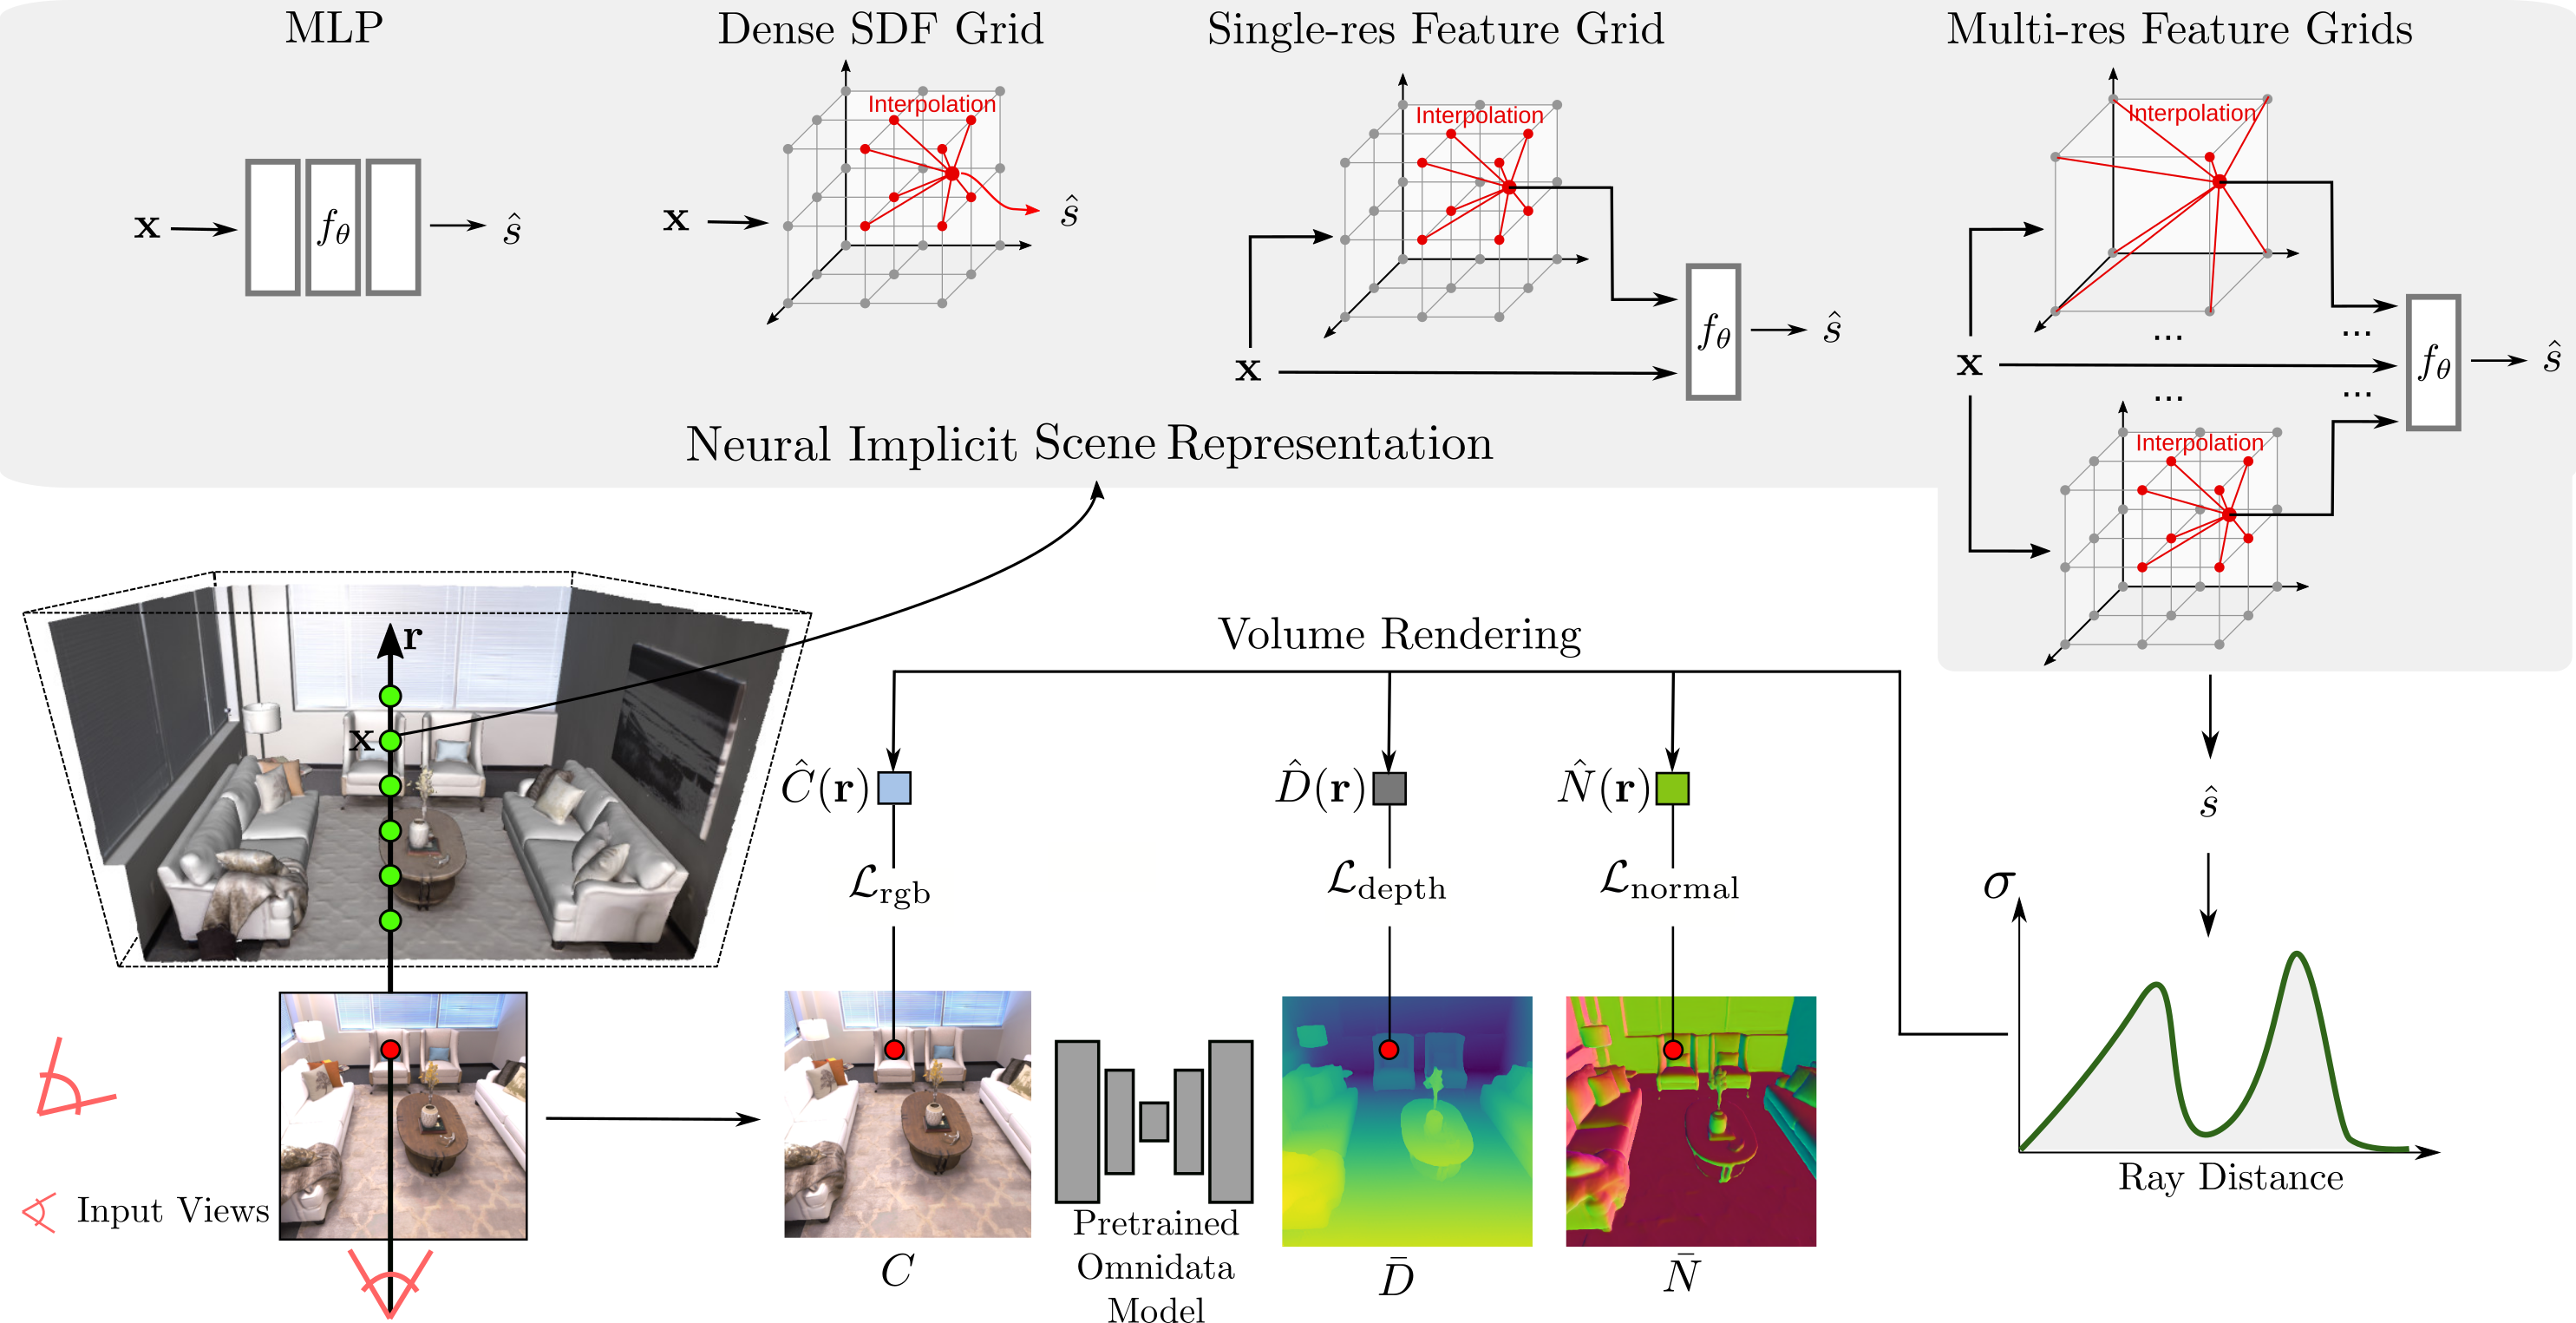
\includegraphics[width=\textwidth]{overview}
    \caption{\textbf{MonoSDF Pipeline.} A batch of rays is randomly sampled and their corresponding color, depth, and normal values are predicted and optimized w.r.t the RGB images, and monocular geometric priors. The method analyzes the different design choices for implicit scene representation by transforming the predicted SDF values to density and then using volume rendering to compute the photometric loss. For simplicity, the color prediction network is not shown here.}
    \label{overview}
    \vspace{-0.4cm}
\end{figure*}

\subsection{Implicit Scene Representations}\label{representation}
The geometry is represented by a continuous signed distance function $f$ as we have discussed in \ref{sdf}. However, the authors of this paper have experimented with several different design choices to parameterize $f$ as mentioned below:
%%
%%
\paragraph{Dense SDF Grid.}  It stores the SDF values directly on the vertices of the discrete SDF grid $\mathcal{G}_\theta$. To compute the SDF value $\hat{s}$ for a 3D point $\mathbf{x}$ it uses $\texttt{interp}$ which is simply tri-linear interpolation.
\begin{equation}
\hat{s} = \texttt{interp}(\mathbf{x}, \mathcal{G}_\theta) \enspace 
\label{eq:dense}
\end{equation}
%%
%%

\paragraph{Single MLP.} The signed distance function $f$ is parameterized by a simple neural network as $f_\theta$. The positional encoding $\gamma$ is computed for 3D point $\mathbf{x}$ and then passed to $f_\theta$ to predict $\hat{s}$.
\begin{equation}
\hat{s} = f_\theta( \gamma(\mathbf{x})) \enspace 
\label{eq:f_mlp}
\end{equation}
%%
%%

\paragraph{Single-Resolution Feature Grid with MLP Decoder.} This simple hybrid method uses MLP $f_\theta$ and and a feature-grid $\Phi_\theta$ combined to parameterize the signed distance function. The MLP $f_\theta$ is conditioned on interpolated features of 3D point $\mathbf{x}$ obtained from $\Phi_\theta$.

\begin{equation}
\hat{s} = f_\theta(\gamma(\mathbf{x}), \texttt{interp}(\mathbf{x}, \Phi_\theta)) \enspace 
\label{eq:single_grid}
\end{equation}

%%
%%
\paragraph{Multi-Resolution Feature Grids with MLP Decoder.} This design approach uses $L$ feature-grids $\{\Phi_\theta^l\}_{l=1}^L$ of different resolutions and then combines those interpolated features to provide condition to $f_\theta$. It helps to combine features at different resolutions to result in a more robust representation. 
\begin{equation}
	\hat{s} = f_\theta(\gamma(\mathbf{x}), \{\texttt{interp}(\mathbf{x}, \Phi_\theta^l)\}_l)) \enspace 
	\label{eq:f_full}
\end{equation}
Note that the number of parameters of feature-grid are independent of the size of the feature-grid because it uses hashing to store the feature vectors in a compact way.
%%
%%

\paragraph{Color Prediction.} The authors used another network $\mathbf{c}_\theta$ to predict the RGB color for the input 3D point $\mathbf{x}$ to optimize the model using photometric reconstruction loss.
\begin{equation}\label{color-mlp}
    \hat{\mathbf{c}} = \mathbf{c}_\theta(\mathbf{x}, \mathbf{v}, \hat{\mathbf{n}}, \hat{\mathbf{z}})
\end{equation}
The color network $\mathbf{c}_\theta$ takes as input a 3D point $\mathbf{x}$, viewing direction $\mathbf{v}$, analytically computed normal vector $\hat{\mathbf{n}}$, and a feature-vector $\hat{\mathbf{z}}$ and predicts the color $\hat{\mathbf{c}}$. Here the feature-vector $\hat{\mathbf{z}}$ is predicted by the second head of the implicit representation network or computed using tri-linear interpolation $\texttt{interp}$ for dense SDF grid.
%%
%%

\subsection{Volume Rendering of Implicit Surfaces}\label{rendering}
%%
%%
\paragraph{SDF-to-Density Transformation.} The RGB images are rendered from implicit representations in order to use photometric consistency loss for optimization. To render an image, the ray is cast from the camera center $\mathbf{o}$ in the viewing direction $\mathbf{v}$ and $M$ point $\mathbf{x}_\mathbf{r}^i = \mathbf{o} + t_\mathbf{r}^i\mathbf{v}$ are sampled along the ray $\mathbf{r}$, and their SDF value $\hat{s}_\mathbf{r}^i$ and RGB value $\hat{\mathbf{c}}^i_\mathbf{r}$ is predicted. This predicted SDF value $\hat{s}_\mathbf{r}^i$ is converted into density $\sigma_\mathbf{r}^i$ using Laplacian CDF following VolSDF \cite{yariv2021volume} to perform volume rendering:
%%
\begin{equation}\label{laplace}
\sigma_\beta(s) = \begin{cases} \frac{1}{2\beta} \exp\left( \frac{s}{\beta} \right) & \text{if } s\leq 0 \\
\frac{1}{\beta}\left( 1-\frac{1}{2}\exp\left ( -\frac{s}{\beta} \right ) \right) & \text{if } s>0
\end{cases} \enspace 
\end{equation}
where $\beta$ is a learnable parameter.
%%
%%

\paragraph{Volume Rendering.} The density $\sigma_\mathbf{r}^i$ is used to render color $\hat{C}(\mathbf{r})$ along the ray $\mathbf{r}$ similar to NeRF \cite{mildenhall2020nerf}:
\begin{align} \label{nerf_color}
\hat{C}(\mathbf{r}) = \sum_{i=1}^M \, T_\mathbf{r}^i \, \alpha_\mathbf{r}^i \, \hat{\mathbf{c}}_\mathbf{r}^i \hspace{1cm}
\end{align}
\begin{equation}
T_\mathbf{r}^i = \prod_{j=1}^{i-1}\left(1-\alpha_\mathbf{r}^j\right)\hspace{1cm}
\alpha_\mathbf{r}^i = 1-\exp\left(-\sigma_\mathbf{r}^i\delta_\mathbf{r}^i\right) \enspace
\label{volume_render}
\end{equation}
where $T_\mathbf{r}^i$ and $\alpha_\mathbf{r}^i$ are transmittance and alpha value of sample $i$ along the ray $\mathbf{r}$. \\

Similarly, depth $\hat{D}(\mathbf{r})$ and normal $\hat{N}(\mathbf{r})$ can also be rendered for a particular ray $\mathbf{r}$:
\begin{equation}
\hat{D}(\mathbf{r}) = \sum_{i=1}^M \, T_\mathbf{r}^i \, \alpha_\mathbf{r}^i \, t_\mathbf{r}^i \hspace{1cm}
\hat{N}(\mathbf{r}) = \sum_{i=1}^M \, T_\mathbf{r}^i \, \alpha_\mathbf{r}^i \, \hat{\mathbf{n}}_\mathbf{r}^i \enspace 
\label{volume_render_dn}
\end{equation}
%%
%%

\subsection{Exploiting Monocular Geometric Cues}\label{cues}
Though implicit scene representation combined with volume rendering works really well, still they struggle to provide high-quality results for texture-less and less observed regions. The problem can be solved by providing the implicit representations with additional geometric priors e.g., depth and normal maps computed by pretrained Omnidata \cite{eftekhar2021omnidata} model.
%%
\paragraph{Monocular Depth Cues.} Given an input RGB image, the depth map $\bar{D}$ can be obtained using the pre-trained model which provides the relative depth. These relative depth cues can provide semi-local relative information and improve the reconstruction quality where there are ambiguities regarding the depth.
\paragraph{Monocular Normal Cues.} Similarly, monocular normal cues $\bar{N}$ can also be computed by using an off-the-shelf model that can provide local geometric details during reconstruction and remove noise.

\begin{figure*}[!htb]
    \centering
    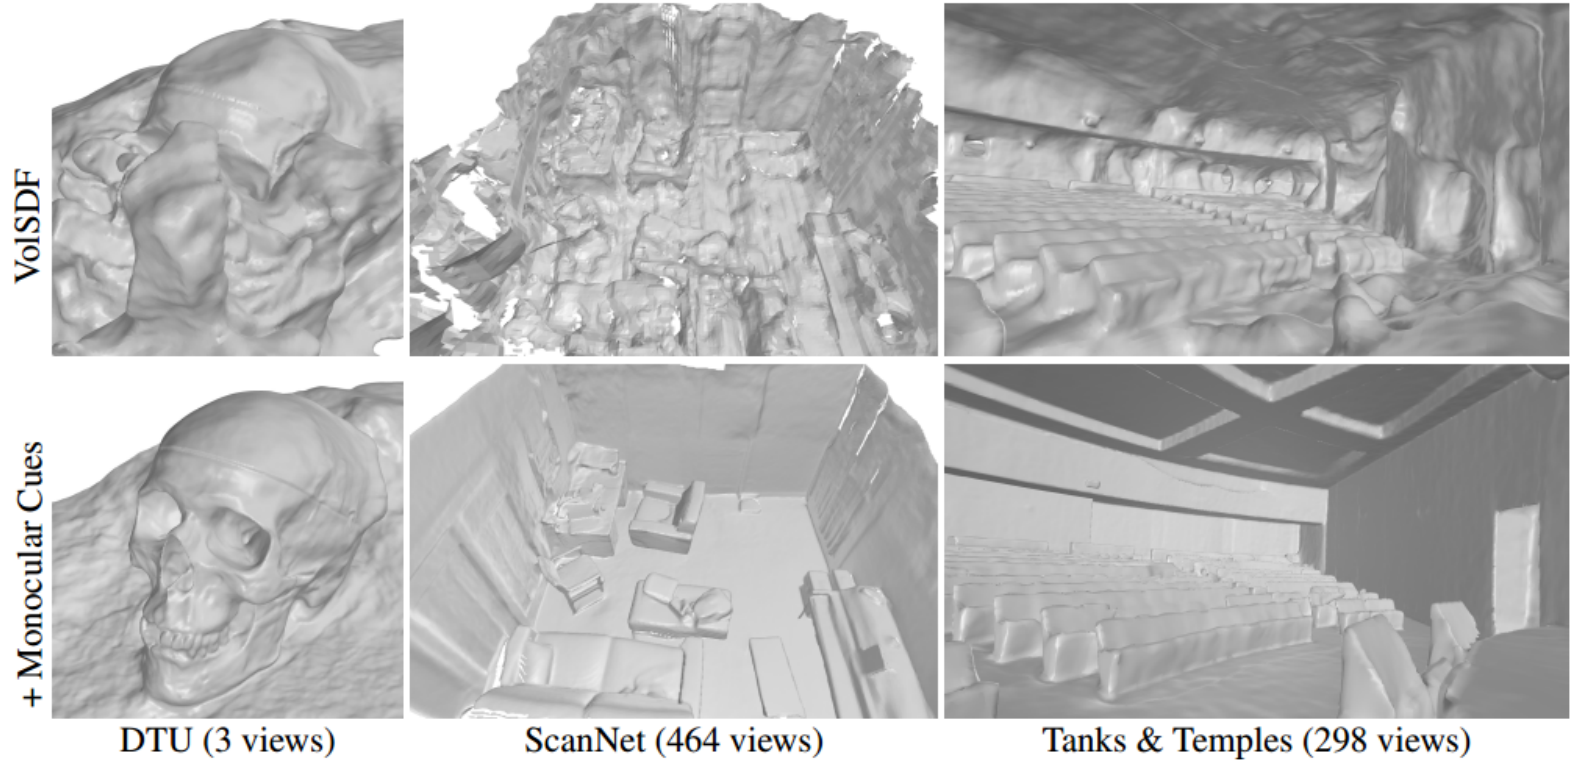
\includegraphics[width=\textwidth]{results}
    \caption{\textbf{MonoSDF Results.} Top: VolSDF completely fails to reconstruct with limited views, and also in case of complex scenes containing multiple objects. Bottom: Implicit scene representations with monocular cues help fill the missing information for sparsely sampled scenes, and remove noise for large-scale scenes.}
    \label{results}
    \vspace{-0.4cm}
\end{figure*}

\subsection{Optimization}\label{optimization}
\paragraph{Reconstruction Loss.} The predicted color $\hat{C}(\mathbf{r})$ from \eqref{nerf_color} is compared with the ground-truth 2D images $C(\mathbf{r})$ to compute RGB reconstruction loss:
\begin{equation}
\mathcal{L}_\text{rgb} = \sum_{\mathbf{r} \in \mathcal{R}} {\lVert \hat{C}(\mathbf{r}) - C(\mathbf{r}) \rVert}_1 \enspace  %
\end{equation}
where $\mathcal{R}$ is a set of rays in the minibatch.

\paragraph{Eikonal Loss.} It regularizes the SDF values of 3D points by enforcing them to satisfy eikonal equation \cite{gropp2020implicit}. i.e., $\lVert \nabla f_\theta(\mathbf{x}) \rVert = \text{1}$.
\begin{equation}
\mathcal{L}_\text{eikonal} = \sum_{\mathbf{x} \in \mathcal{X}} ({\lVert \nabla f_\theta(\mathbf{x}) \rVert}_2 - 1)^2 \enspace
\end{equation}
Here $\mathcal{X}$ is joint set of uniformly sampled points and points near the surface.

\paragraph{Depth Consistency Loss.} Rendered depth maps $\hat{D}(\mathbf{r})$ are compared with the predicted depth maps $\bar{D}$ to compute depth consistency loss:
\begin{equation}
\mathcal{L}_\text{depth} = \sum_{\mathbf{r} \in \mathcal{R}} {\lVert (w \hat{D}(\mathbf{r}) + q) - \bar{D}(\mathbf{r}) \rVert}^2 \enspace  \label{depth_loss}
\end{equation}
where $w$ and $q$ are scale and shift factors to align rendered and predicted depth maps $\hat{D}$ and $\bar{D}$ respectively. These $w$ and $q$ are computed analytically separately for each batch of rays.

\paragraph{Normal Consistency Loss.} Similarly, the L1 loss and angular loss is computed for rendered normal $\hat{N}$ and predicted normal $\bar{N}$ to enforce normal consistency:
\begin{equation}
\mathcal{L}_\text{normal} = \sum_{\mathbf{r} \in \mathcal{R}} {\lVert \hat{N}(\mathbf{r}) - \bar{N}(\mathbf{r}) \rVert}_1 +  {\lVert  1 - \hat{N}(\mathbf{r})^\top  \bar{N}(\mathbf{r}) \rVert}_1 \enspace 
\end{equation}

The overall loss used for optimization is a weighted sum of these individual losses:
\begin{equation}
    \mathcal{L} = \mathcal{L}_{\text{rgb}} + \lambda_1 \mathcal{L}_\text{eikonal} + \lambda_2\mathcal{L}_{\text{depth}} + \lambda_3\mathcal{L}_{\text{normal}} \enspace 
\end{equation}
where $\lambda_1$, $\lambda_2$, $\lambda_3$ are weight factors with values 0.1, 0.1, 0.05 respectively.

\section{Results}
The authors evaluated their model on four datasets: DTU (object-level scenes), Replica and ScanNet (real-world indoor scans), Tanks and Temples (large-scale indoor scenes). They reported the result for different choices of implicit neural scene representations and studied the effect of monocular geometric priors. For Replica, they highlighted that monocular cues improve results for both kinds of architectures grids as well as MLPs, however, feature-grids increase optimization speed while MLPs result in better accuracy. \newline

For the ScanNet dataset, the images of the scenes are blurry and camera poses are also noisy. However, MLPs with monocular cues produce very good reconstructions shown in \figref{results} because of their inductive smoothness bias. Similarly, neural implicit scene representations combined with monocular priors perform really well on Tanks and Temples dataset (see \figref{results}) which consists of huge indoor scenes. The authors claim that MonoSDF is the first method that can provide smooth reconstructions on this dataset. \newline

They also evaluated their method in a sparse view (3 views) setting with DTU dataset. In \figref{results}, we can see few-shot reconstruction for DTU provided complete reconstructions for objects in the scene because of additional supervision signal provided by monocular cues. However, they also highlighted the failure case when the object is duplicated in front of each camera frustum. They hinted that this issue can be resolved by providing a sparse point cloud as an additional constraint during training.

\section{Discussion \& Conclusion}
We have seen MonoSDF improves the 3D reconstruction and also reduces the optimization time by incorporating monocular geometric priors during the training of neural implicit scene representations. However, it is dependent on an off-the-shelf model that can predict depth and normal maps for the 2D scene images. Omnidata \cite{eftekhar2021omnidata} generalizes really well across the scenes, however, it only accepts images with low-resolutions ($384 \times 384$ pixels) but most of the real-world scenes have higher-resolutions and downsizing the images results in loss of performance. Though the authors have experimented with creating higher-resolution monocular cues in a sliding window manner over the image but they believe that it is not the best way to solve this issue. \\

In summary, this work investigated the different design choices for neural implicit scene representations, studied the effect of using monocular geometric priors, and experimented with a wide variety of datasets. It showed how monocular cues can improve the 3D reconstruction for large-scale scenes and less-observed regions. However, we have also discussed a failure case where the object is duplicated in front of each camera frustum. The authors hinted that the results can further be improved by using occlusion edges, planes, and curvature cues during training. They also suggested another interesting research direction to optimize scene representations and camera parameters jointly which will reduce the effect of motion blur and noisy camera poses. \\

Apart from this, recognition cues from classifiers can also be utilized during the training of implicit scene representations. The pretrained image classifiers are provided with a lot of augmented and multi-view image data that enables them to classify an object from almost every possible angle. If we extract that knowledge from CNNs or ViTs and provide it to the neural implicit scene representations we can further reduce the reconstruction errors, however, providing this knowledge to implicit scene representations is challenging.
%% <--------------------------------------------------------------
%% <--------------------------------------------------------------
\bibliographystyle{plain}
\bibliography{references}

\end {document}
